% ----------------------------------------------------------------------

\newpage

\subsection{\scurves Test}
\label{ss:scurves}

\subsubsection{Purpose}

The \scurves test as configured for FPix module testing has two primary purposes.
First, it evaluates the efficacy of the \trimming test.
Secondly, it measures the noise present in each pixel and can potentially flag abnormally noisy pixels.
Both of these goals are achieved by fitting the curve of efficiency vs. \vcal for each pixel.
The test gets its name from the shape of the error function used to fit the measured curve.

\subsubsection{Methodology}

An \scurves test is a generic type of test that measures a pixel's efficiency as a function of a chosen \dac.
Assuming the pixel will not respond at low values of the \dac in question and will be fully efficient at some higher value of the \dac,
the efficiency curve should have a region of zero efficiency, 
a transition region with increasing efficiency, and a plateau region with 100\% efficiency.
The shape of this curve mildly resembles the letter ``S''.
If no noise is present in the system the turn-on curve will be a simple step function, 
with the horizontal floor and plateau connected by a vertical line.
However, noise will reduce the slope of the line connecting the floor and plateau.
Using this fact, an estimate of the noise in the system can be extracted from the width of the turn-on curve.

For each pixel, the s-curve is fit with an error function, which is the cumulative distribution function for a Gaussian curve.
From this curve, three parameters are extracted.
The turn-on threshold, defined as the \dac value at which 50\% efficiency is reached, is denoted by the shorthand ``thr''.
The width of the turn-on curve, defined as the width parameter of the fitted error function, is denoted by the shorthand ``sig''.
Finally, the turn-off threshold, 
defined as the point above the turn-on threshold at which efficiency drops back below 50\%, is denoted by the shorthand ``thn''.

For the \scurves test as configured for FPix module testing, 
an \scurves test is performed over \vcal, in a \vcal range window around the target threshold for the \trimming test.
This is because, post-trimming, the expected region of the turn-on of the s-curve is known.
The number of triggers is configurable, but in order to extract accurate width values, 
a large number of triggers (default is 200) should be used.

\subsubsection{Output}

Figures~\ref{fig:scurves_thr_scurveVcal_Vcal}-\ref{fig:scurves_dist_thn_scurveVcal_Vcal} 
show the output of the \scurves test as used in the \fulltest for FPix module qualification.
\roc maps and 1D distributions of the three parameters measured by the test are saved in the output file: 
the turn-on ``thr'' (Figures~\ref{fig:scurves_thr_scurveVcal_Vcal},~\ref{fig:scurves_dist_thr_scurveVcal_Vcal}),
the width ``sig'' (Figures~\ref{fig:scurves_sig_scurveVcal_Vcal},~\ref{fig:scurves_dist_sig_scurveVcal_Vcal}),
and the turn-off ``thn'' (Figures~\ref{fig:scurves_thn_scurveVcal_Vcal},~\ref{fig:scurves_dist_thn_scurveVcal_Vcal}).
For s-curves with respect to \vcal, no turn-off is expected (it's mainly useful for \vthrcomp s-curves).
When no turn-off is observed, the test returns the maximum value of the \dac in question that is tested.

\begin{figure}[!htp]
\centering
\begin{minipage}{0.45\textwidth}
  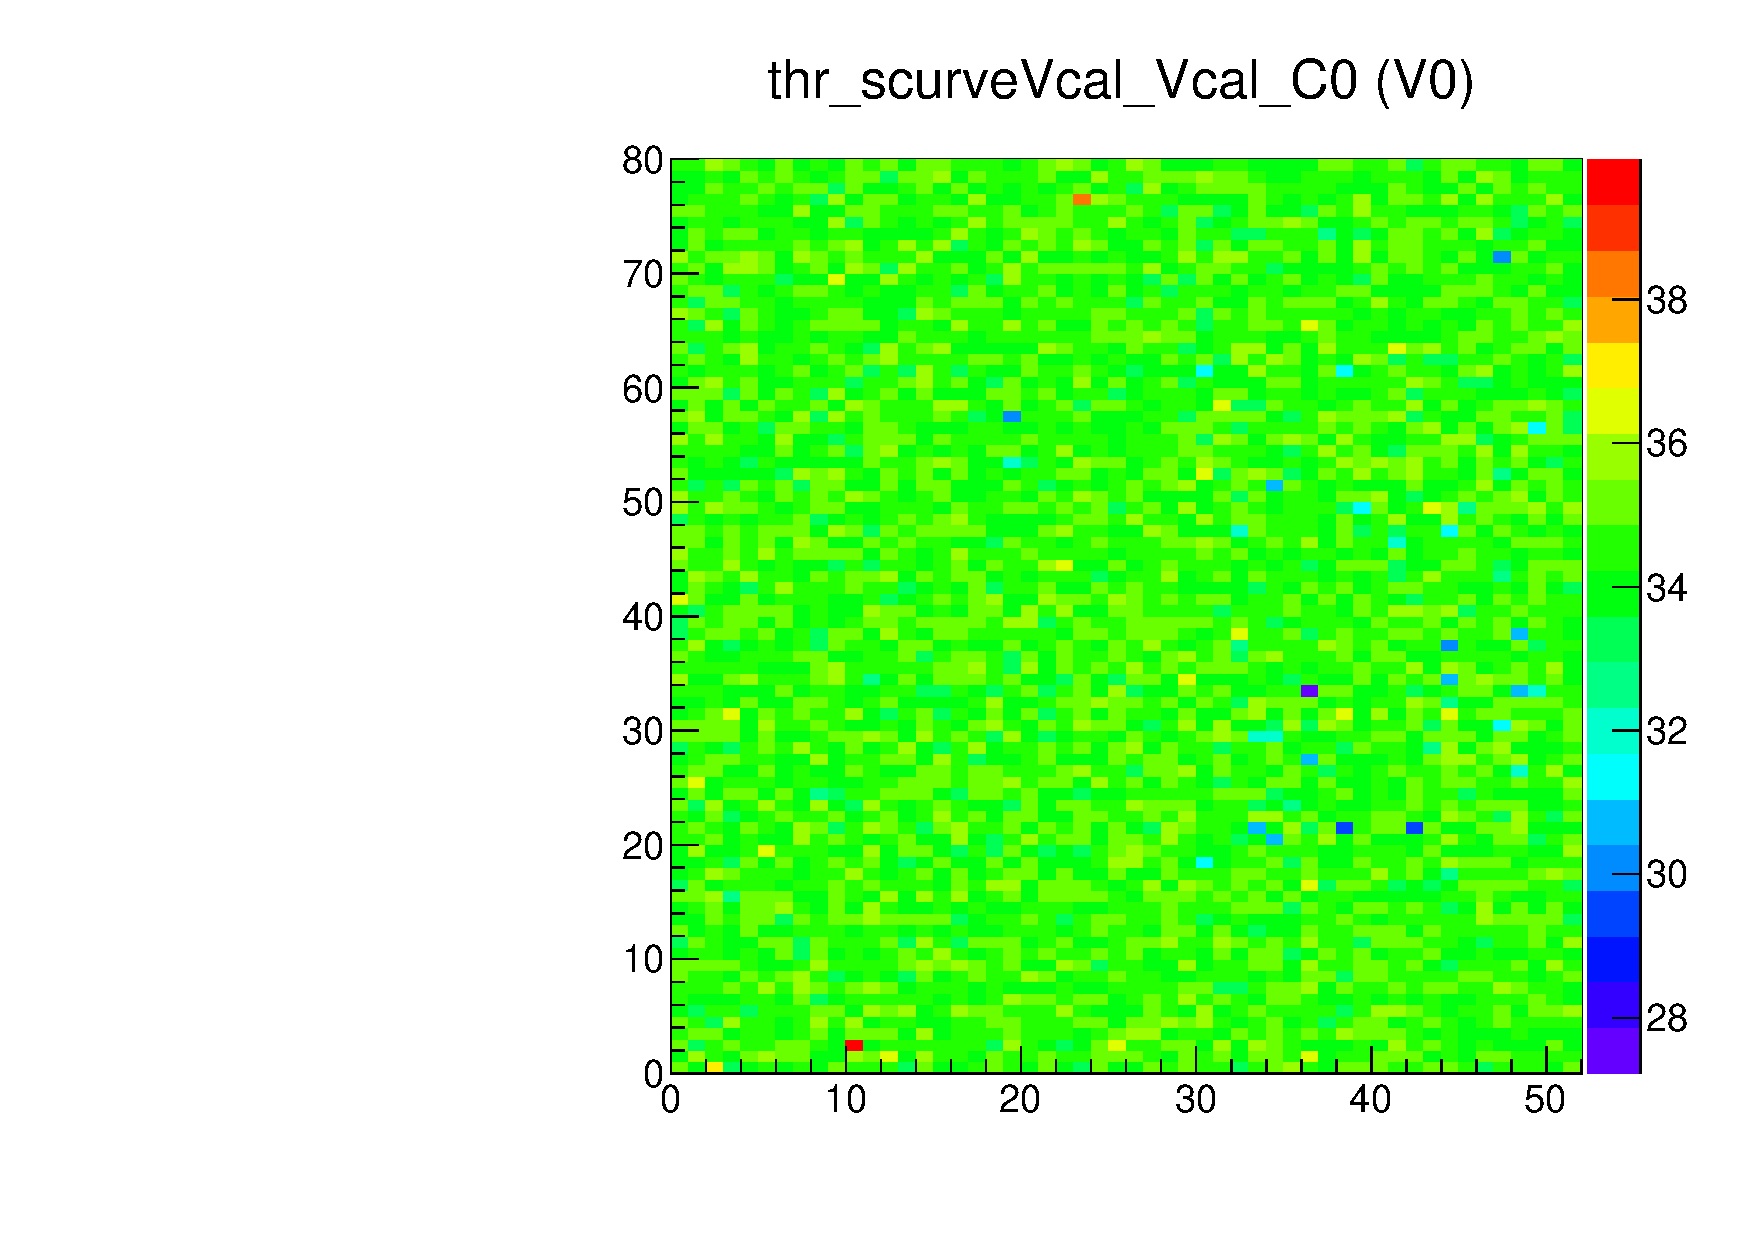
\includegraphics[width=1.0\textwidth]{figures/scurves_thr_scurveVcal_Vcal.pdf}
  \caption{\roc map of the \vcal s-curve turn-on thresholds.
  Values should be near the trim target (default 35).}
  \label{fig:scurves_thr_scurveVcal_Vcal}
\end{minipage}
\hspace{0.3cm}
\begin{minipage}{0.45\textwidth}
  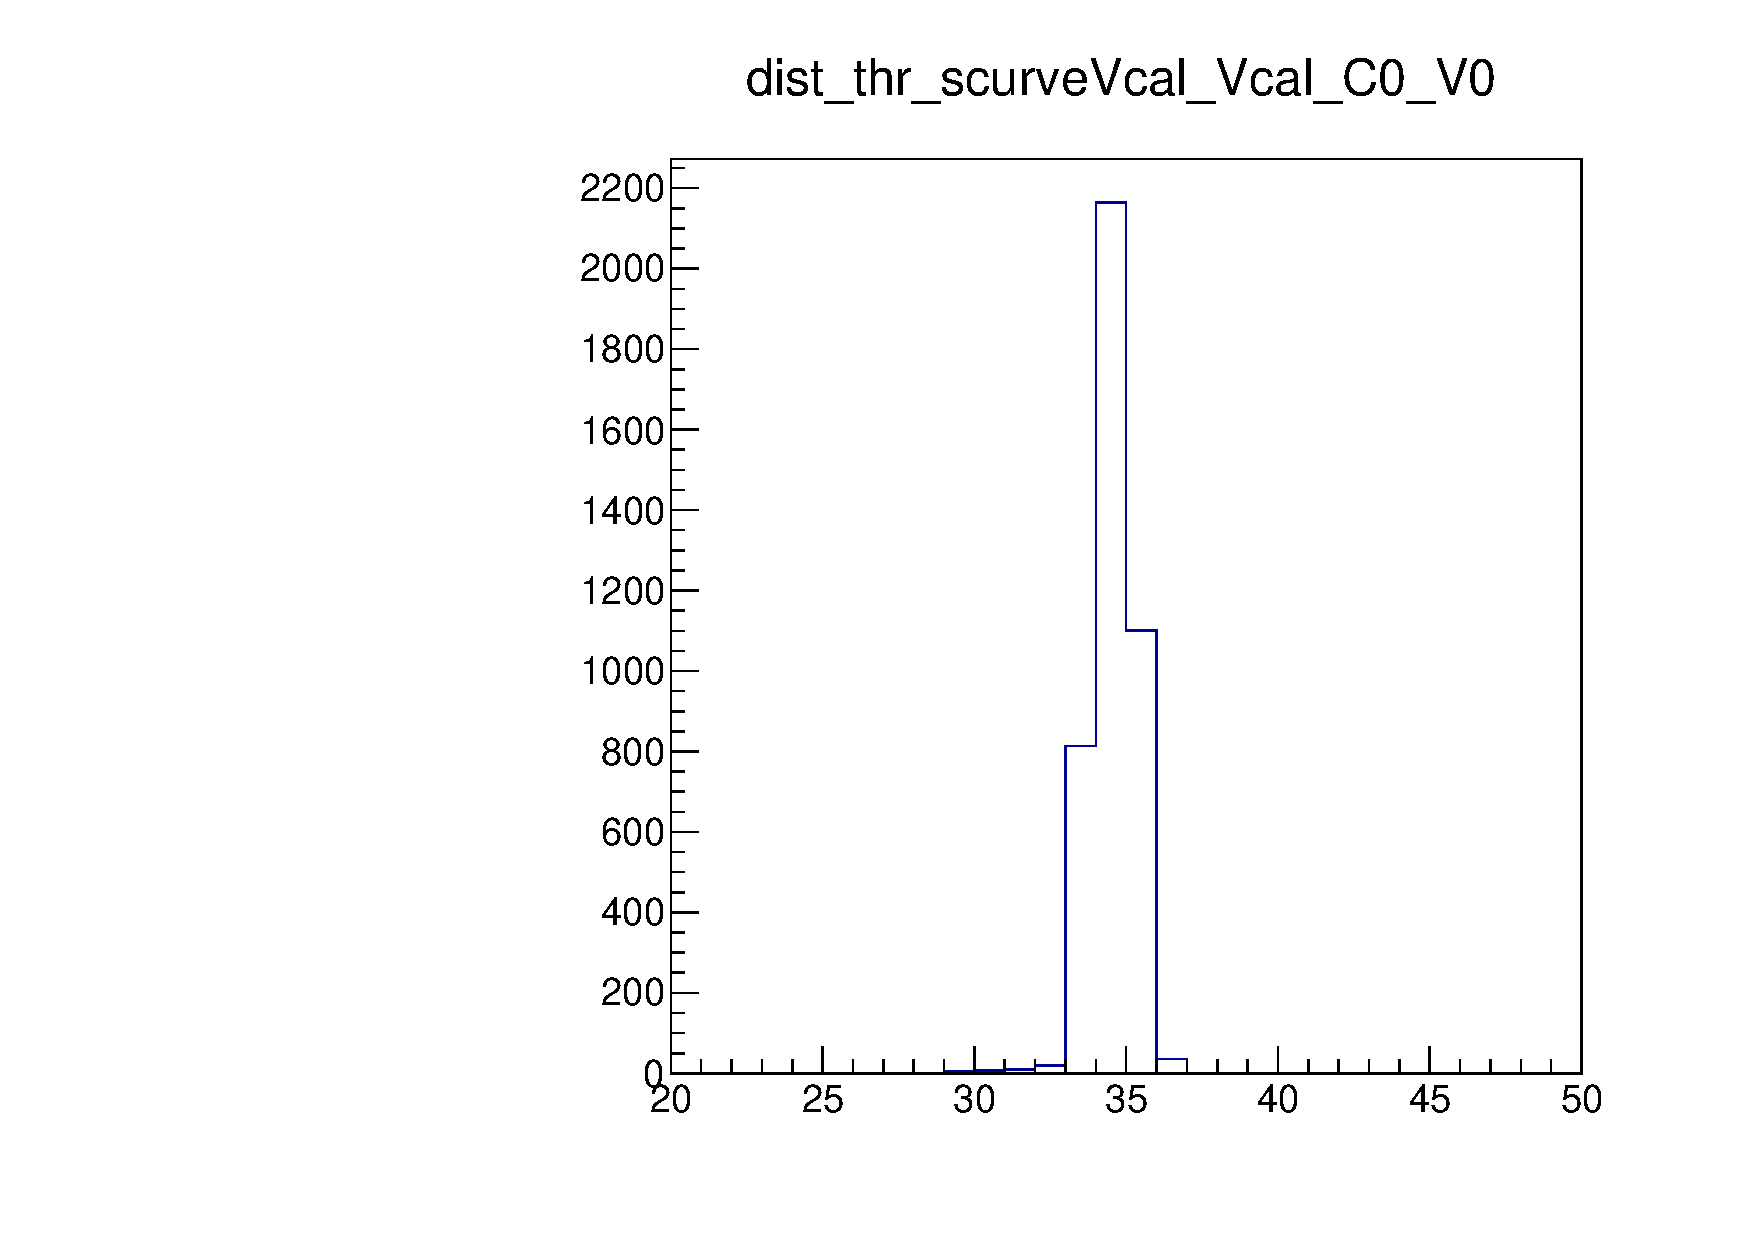
\includegraphics[width=1.0\textwidth]{figures/scurves_dist_thr_scurveVcal_Vcal.pdf}
  \caption{1D distribution of Figure~\ref{fig:scurves_thr_scurveVcal_Vcal}.
  [original range 0-255]}
  \label{fig:scurves_dist_thr_scurveVcal_Vcal}
\end{minipage}
\end{figure}

\begin{figure}[!htp]
\centering
\begin{minipage}{0.45\textwidth}
  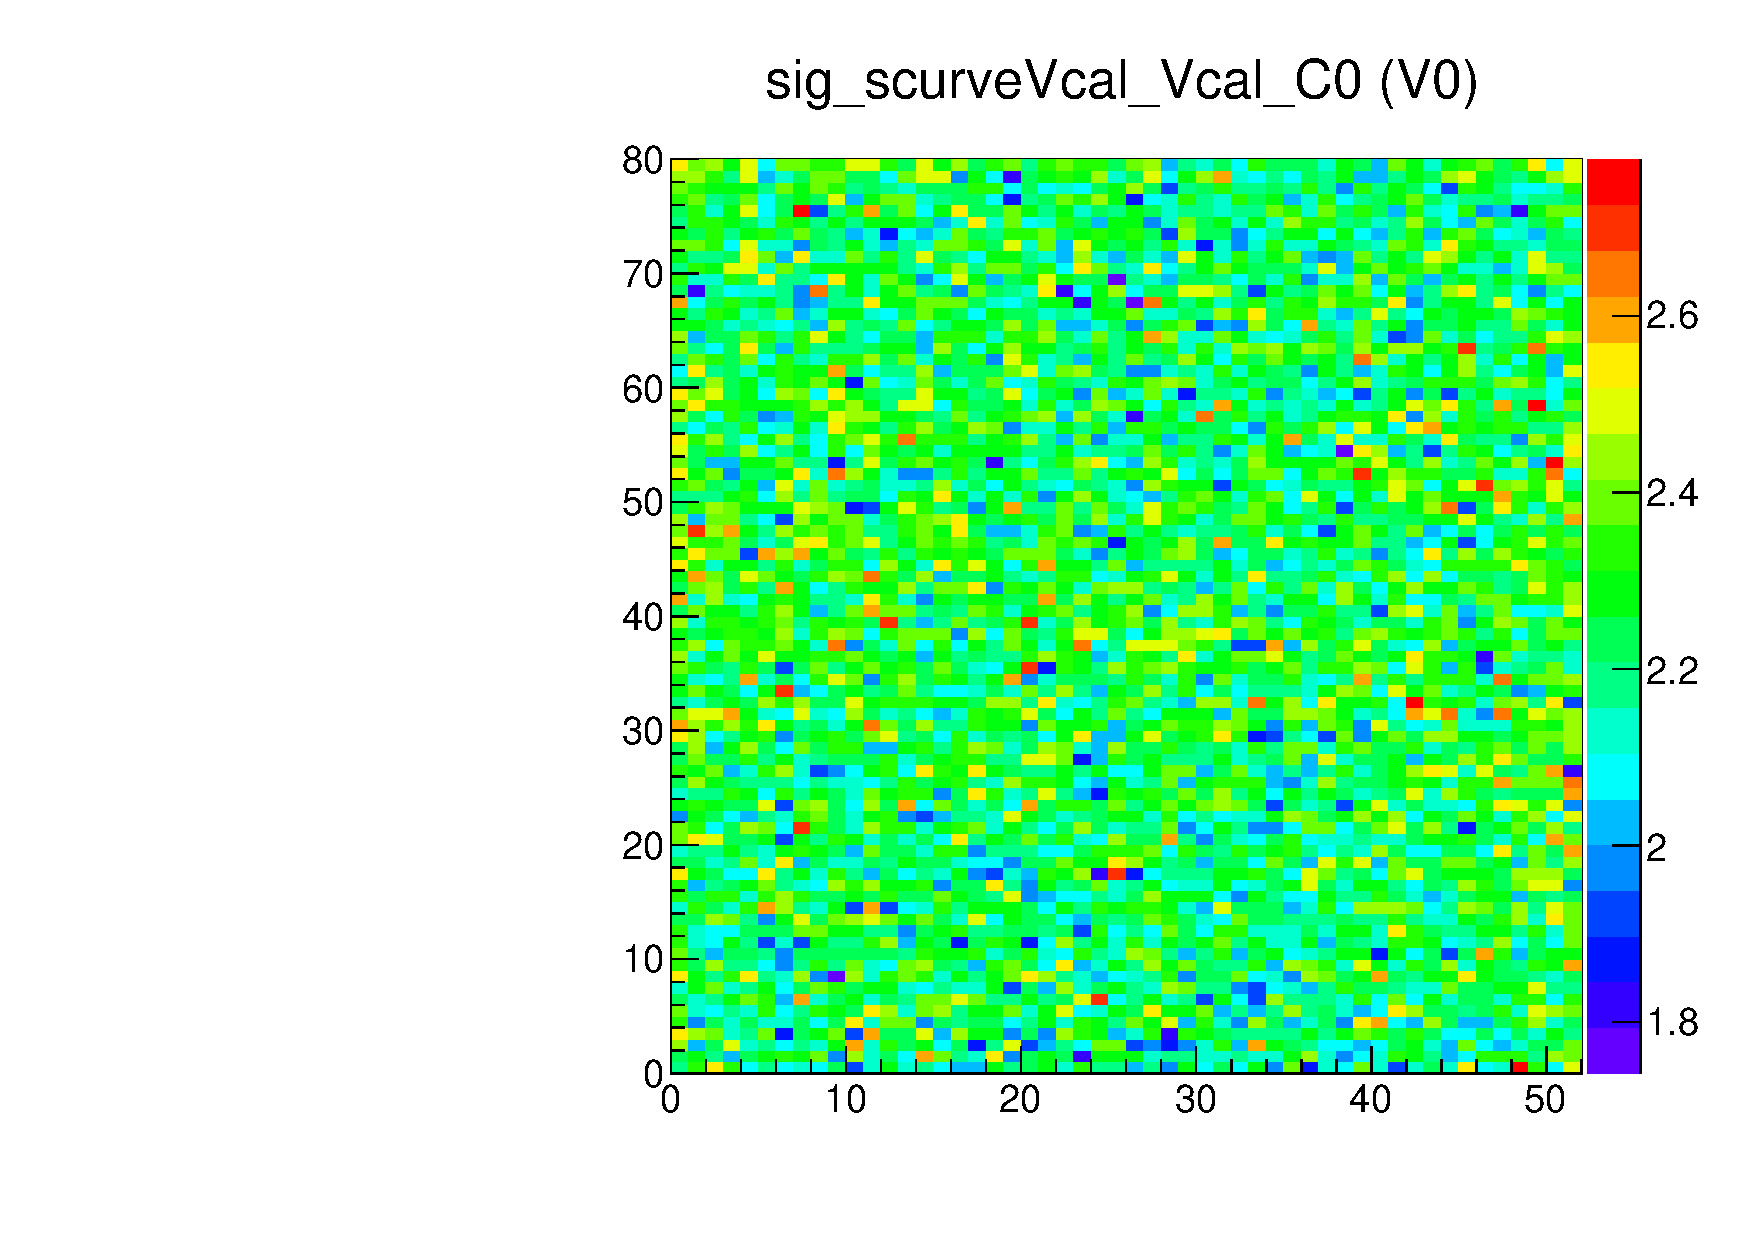
\includegraphics[width=1.0\textwidth]{figures/scurves_sig_scurveVcal_Vcal.pdf}
  \caption{\roc map of the \vcal s-curve turn-on widths.  
  This width is proportional to the noise in the system.}
  \label{fig:scurves_sig_scurveVcal_Vcal}
\end{minipage}
\hspace{0.3cm}
\begin{minipage}{0.45\textwidth}
  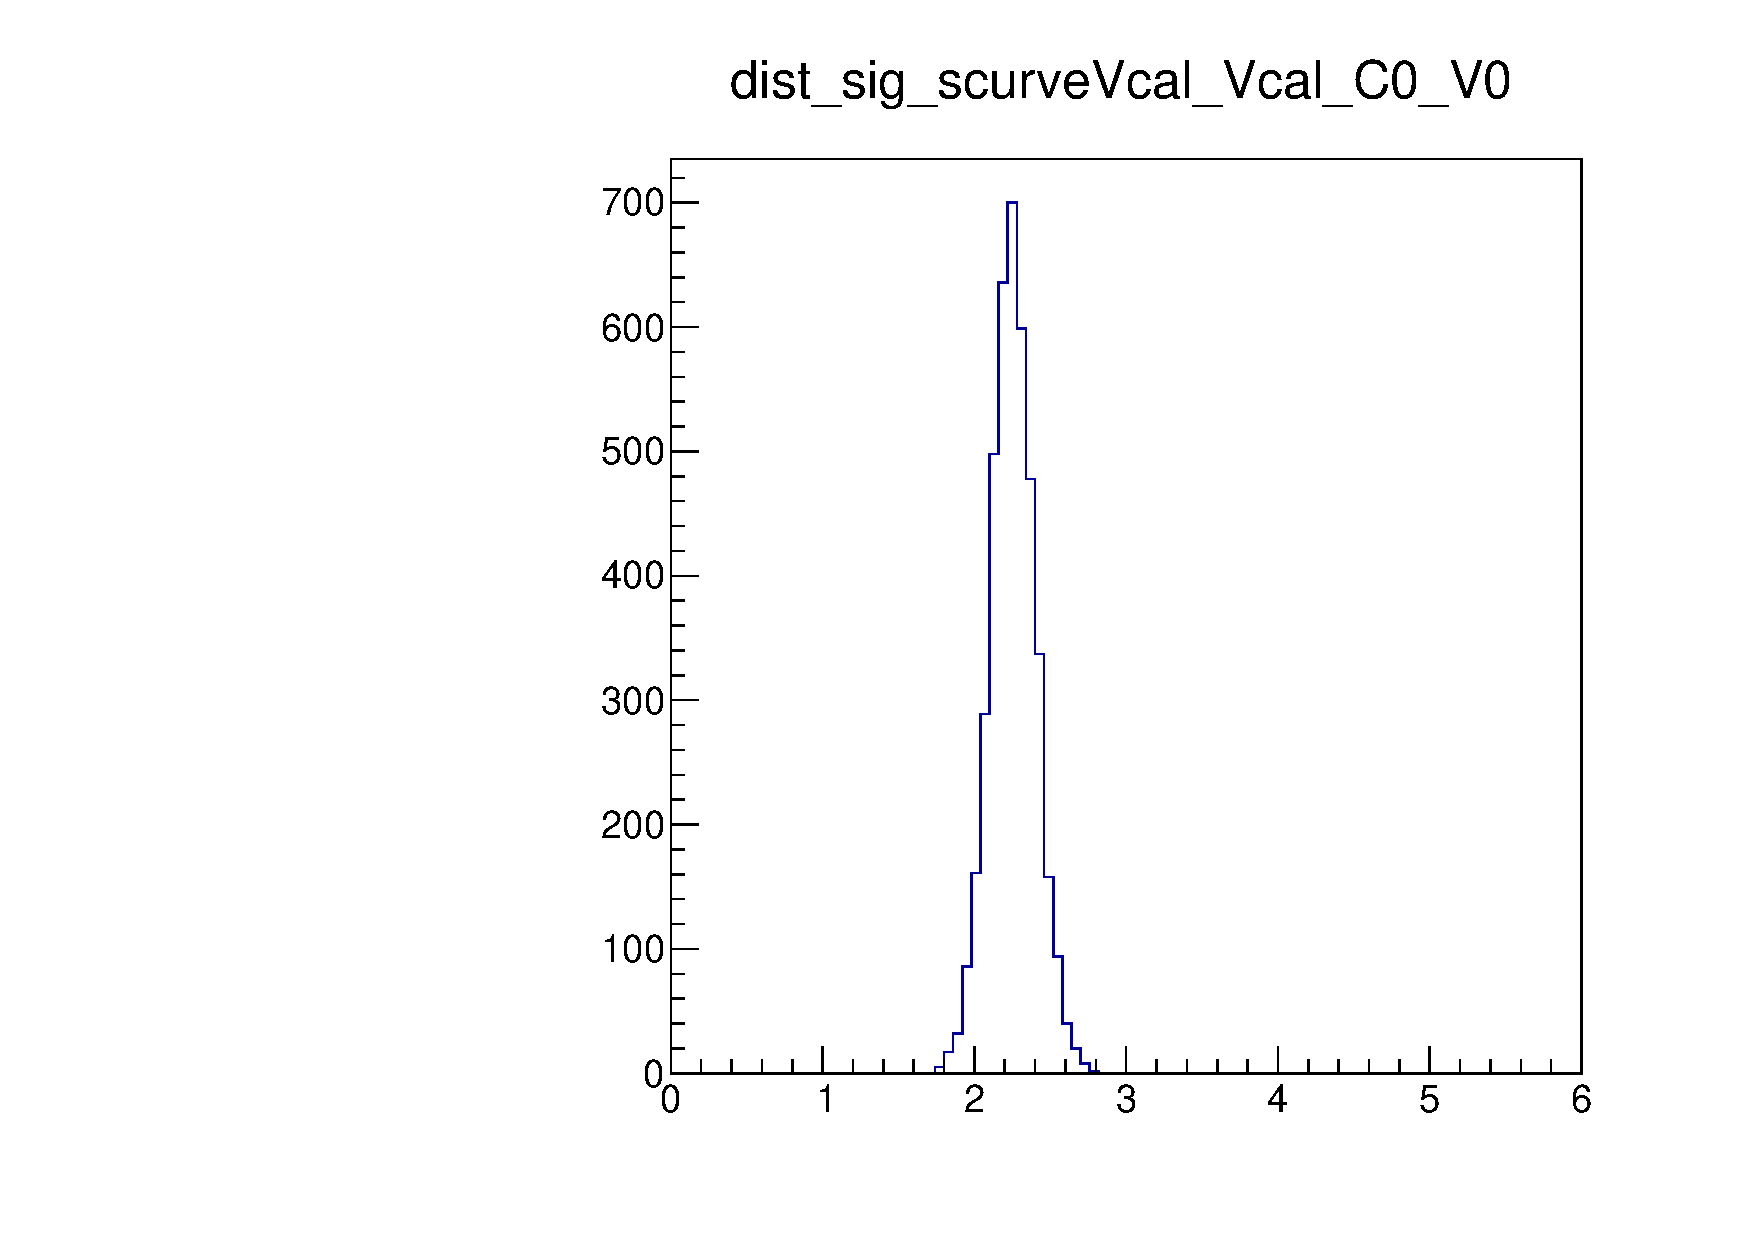
\includegraphics[width=1.0\textwidth]{figures/scurves_dist_sig_scurveVcal_Vcal.pdf}
  \caption{1D distribution of Figure~\ref{fig:scurves_sig_scurveVcal_Vcal}.}
  \label{fig:scurves_dist_sig_scurveVcal_Vcal}
\end{minipage}
\end{figure}

\begin{figure}[!htp]
\centering
\begin{minipage}{0.45\textwidth}
  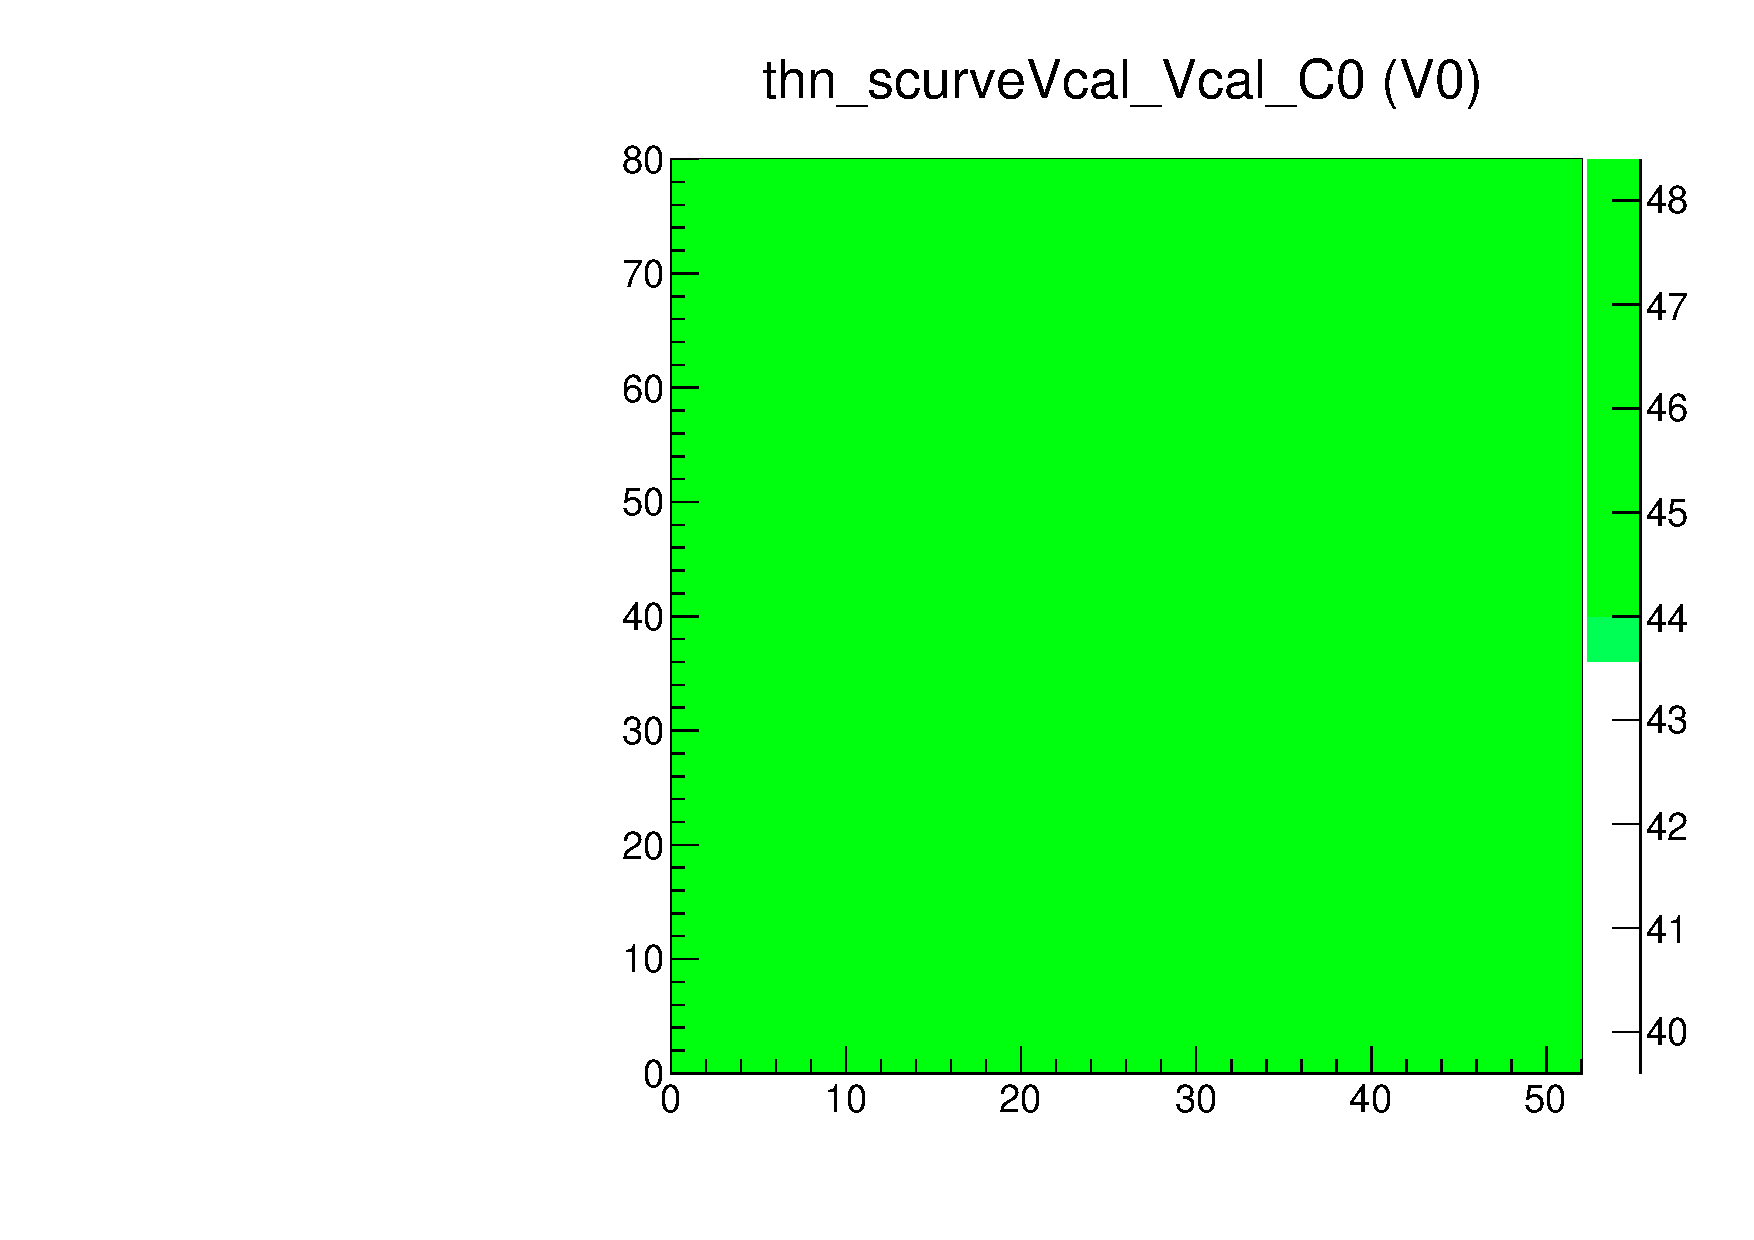
\includegraphics[width=1.0\textwidth]{figures/scurves_thn_scurveVcal_Vcal.pdf}
  \caption{\roc map of the \vcal s-curve turn-off thresholds.  
  For s-curves with respect to \vcal, no turn off is expected.
  Therefore this plot should be uniformly distributed at the maximum value of \vcal considered by the test.}
  \label{fig:scurves_thn_scurveVcal_Vcal}
\end{minipage}
\hspace{0.3cm}
\begin{minipage}{0.45\textwidth}
  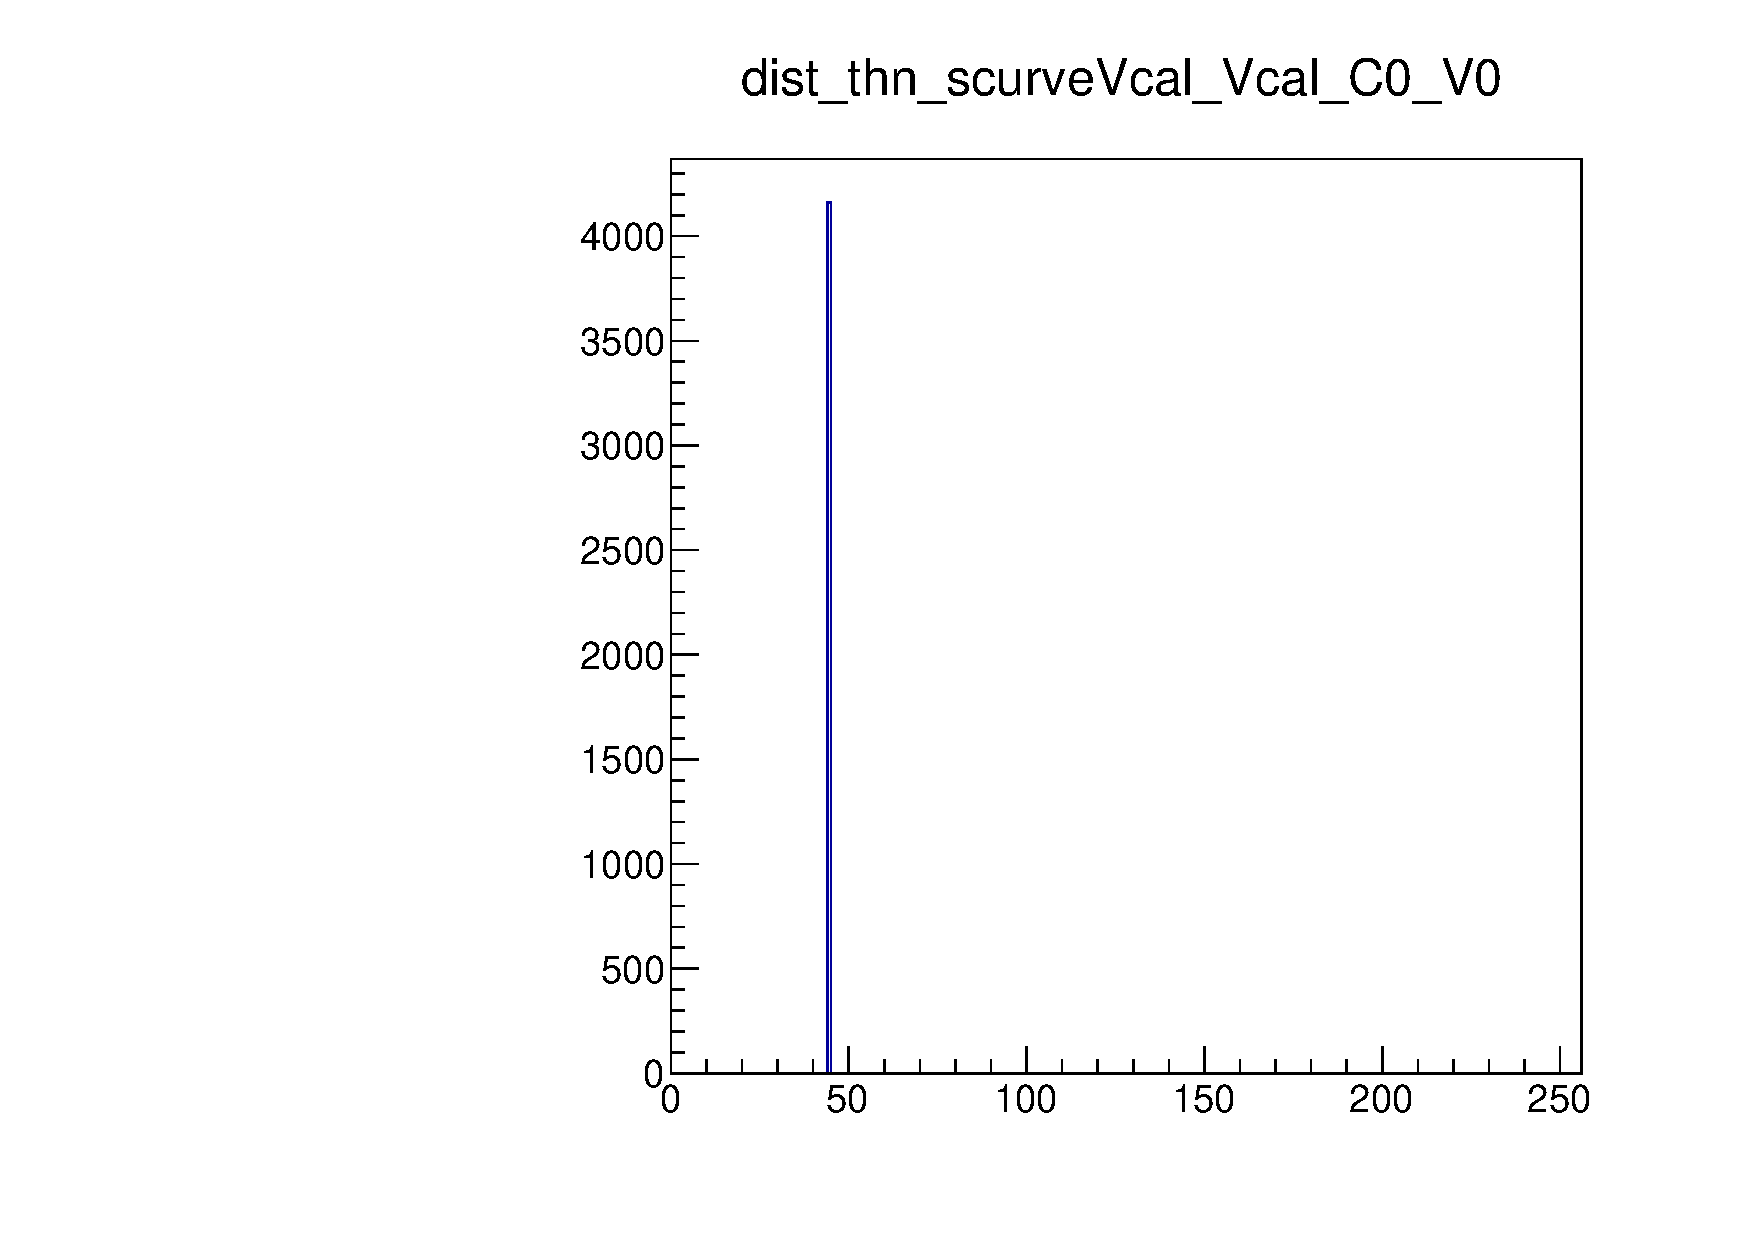
\includegraphics[width=1.0\textwidth]{figures/scurves_dist_thn_scurveVcal_Vcal.pdf}
  \caption{1D distribution of Figure~\ref{fig:scurves_thn_scurveVcal_Vcal}.}
  \label{fig:scurves_dist_thn_scurveVcal_Vcal}
\end{minipage}
\end{figure}


